%!TEX root = thesis.tex

\chapter{Follow-Up User Study}
\label{chap:follow-up-user-study}

A follow-up user study was conducted to evaluate the set of refined visualisations. In addition to evaluating this iteration of the visualisation prototype, the limitations identified in the first user study were also to be addressed. This included providing a valid baseline for the study (the \emph{no visualisation} condition) and reducing the visualisations to more meaningful representations.

\section{Method}

Two independent audiences ($N=14+11=25$) were recruited through on campus advertisement (see Appendix~\ref{appendix:follow-up-user-study-advertisement}). Each group was exposed to two live coding musical performances. One of the performances displayed only the source code of the performance while the other displayed the source code with a visualisation underlay (see Chapter~\ref{chap:visualisation-refinement}).

It was hypothesised that the visualisation prototype would result in higher understanding at the end of the performance and that enjoyment would remain steady throughout both performances.

The first group was subjected to the \emph{visualisation} condition, followed by the \emph{no visualisation} condition. The conditions were swapped for the second group, with the audience exposed to the \emph{no visualisation} condition first followed by the \emph{visualisation} condition.

\section{Participants}

Of the 25 total participants over the two performances $12\%$ were female. $64\%$ of the audience had not been to a live coding performance before and $80\%$ had not attended the previous live coding user study. The background of the audience included $56\%$ that listened to music regularly, $28\%$ that played an instrument and $72\%$ who programmed for their hobby, job or study.

\section{Results}

The audience-reported enjoyment and understanding responses from the survey were evaluated for the two conditions as described below.

\subsection{Enjoyment}

$60\%$ of the audience stated that projection of the code helped their enjoyment of the performance directly while $16\%$ of the audience stated that the visualisations helped their enjoyment directly.

\afterpage{
\begin{figure}
  \centering
  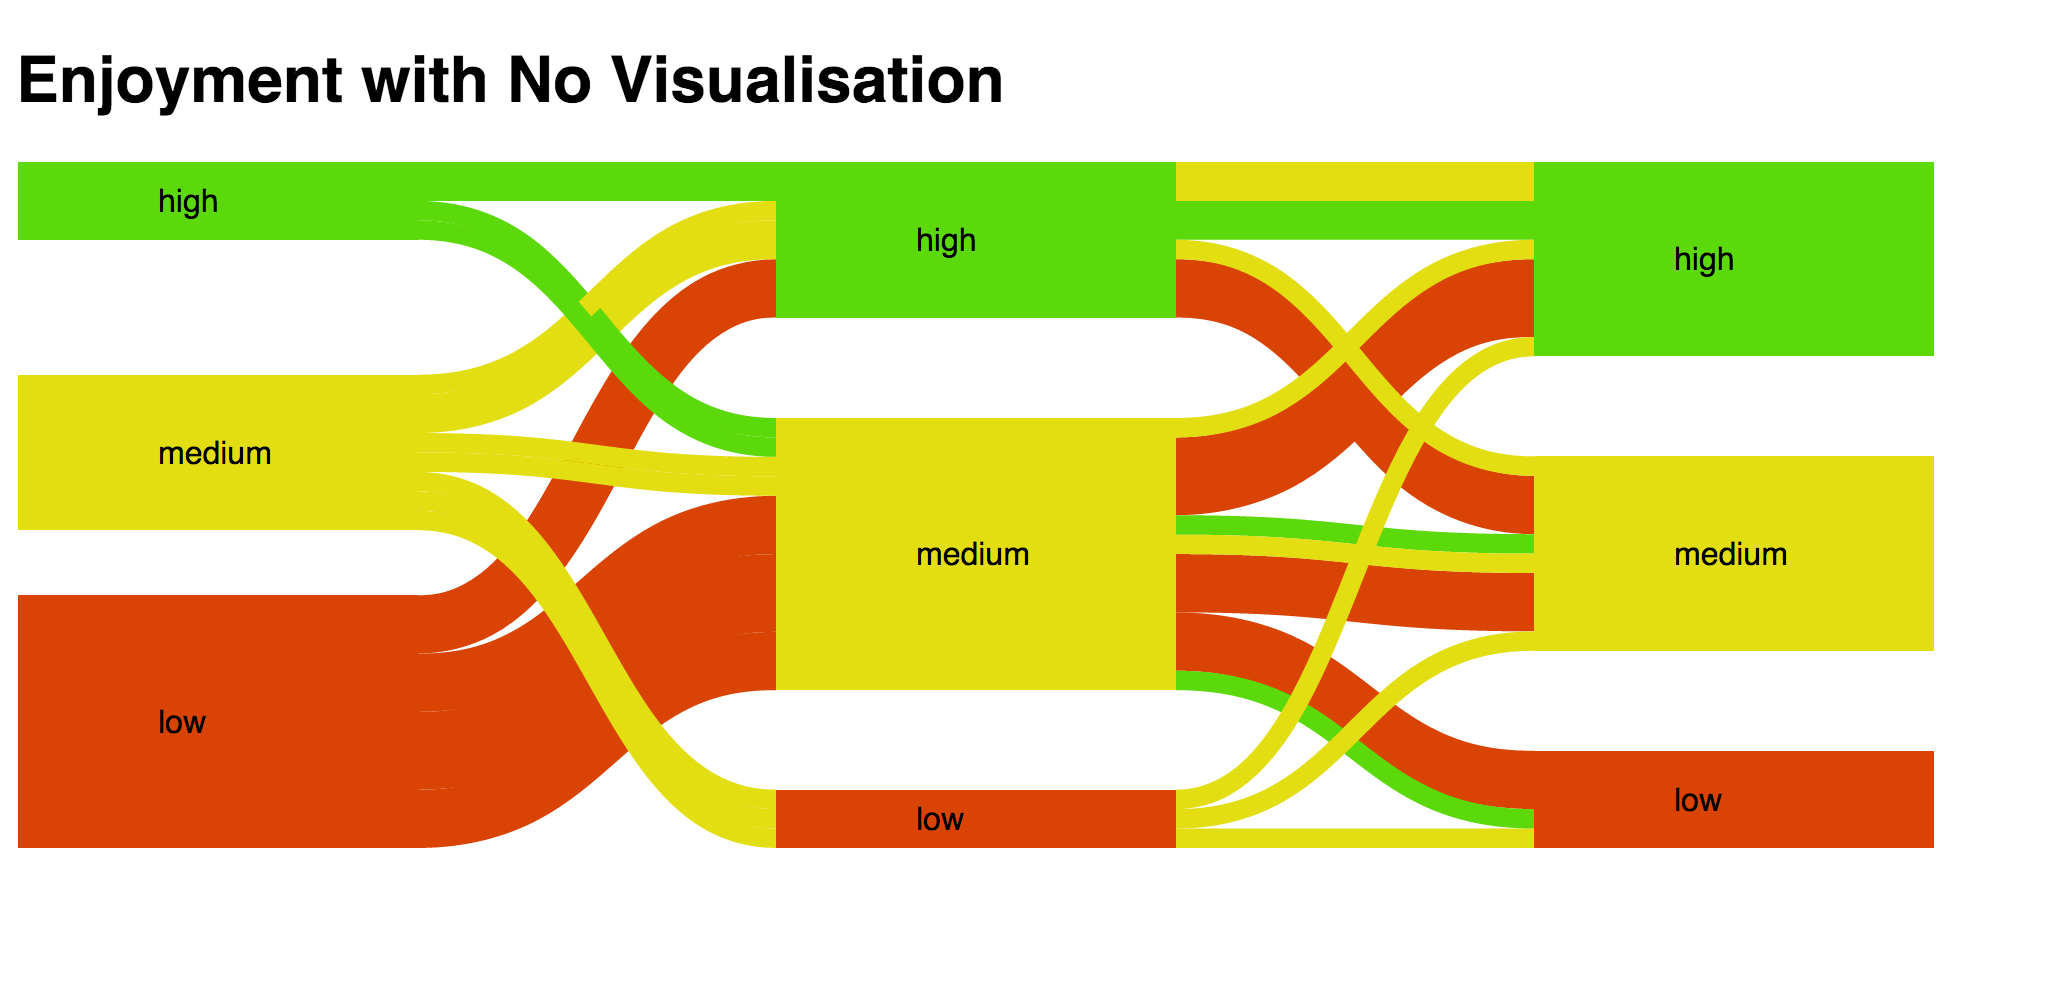
\includegraphics[width=\columnwidth]{../study-3/results/enjoyment-with-no-visualisation-study-3}
  \caption{Audience reported enjoyment during the beginning, middle and end of the performance with \textbf{no} visualisations. Line width at each stage indicates proportion of the audience reporting high, medium or low enjoyment, and line colour is determined by the enjoyment level at the \emph{beginning} of the performance.}
  \label{fig:no-visualisations-enjoyment}
\end{figure}

\begin{figure}
  \centering
  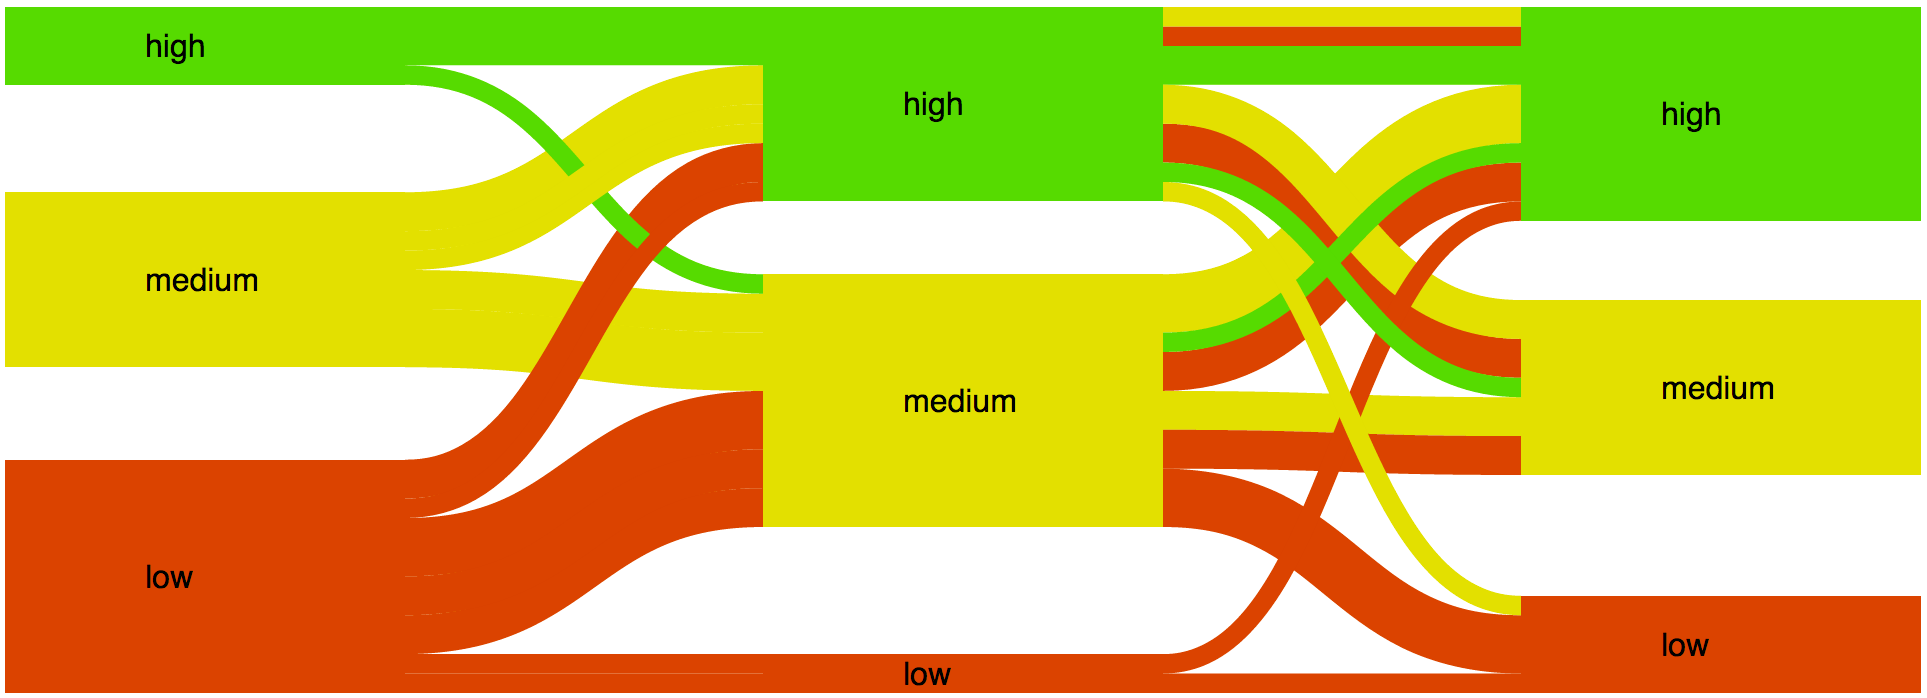
\includegraphics[width=\columnwidth]{../study-3/results/enjoyment-with-visualisation-study-3}
  \caption{Audience-reported enjoyment level during the beginning, middle and end of the performance with visualisations.}
  \label{fig:visualisations-enjoyment}
\end{figure}
\clearpage}

\subsection{Understanding}

$76\%$ of the audience stated that projection of the code helped their understanding of the performance directly while $32\%$ of the audience stated that the visualisations helped their understanding directly.

\afterpage{
\begin{figure}
  \centering
  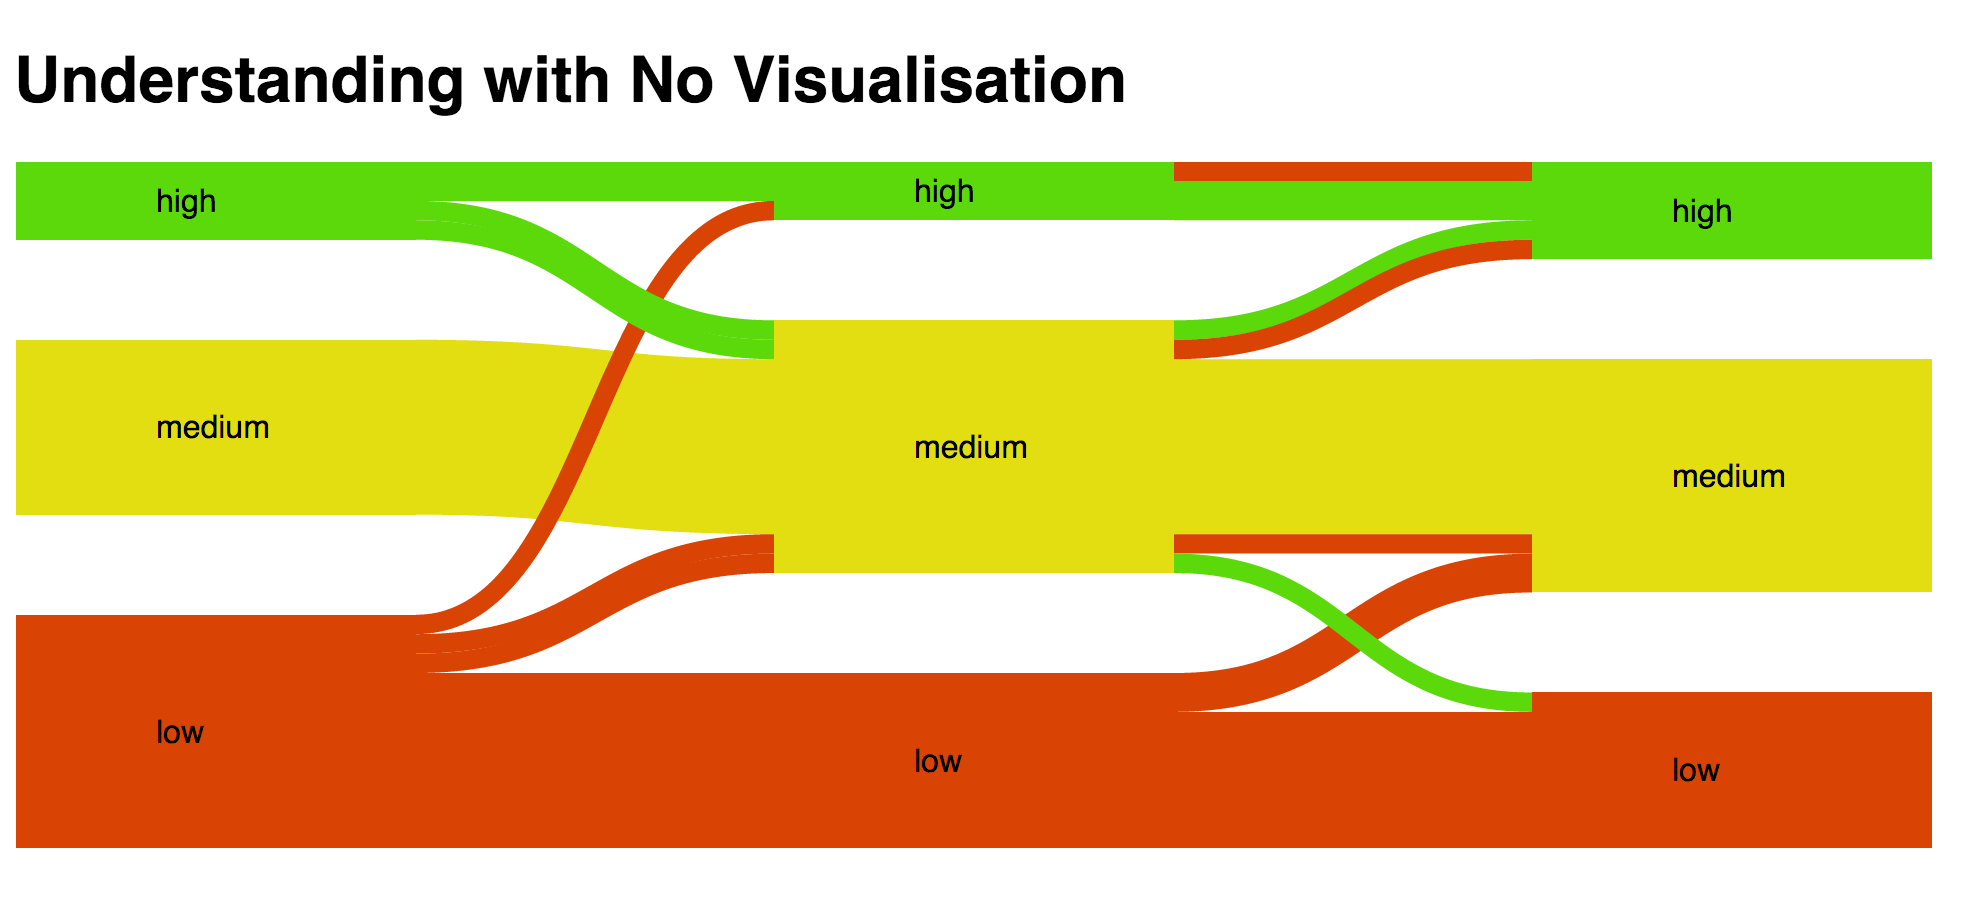
\includegraphics[width=\columnwidth]{../study-3/results/understanding-with-no-visualisation-study-3}
  \caption{Audience reported understanding during the beginning, middle and end of the performance with \textbf{no} visualisations.}
  \label{fig:no-visualisations-understanding}
\end{figure}

\begin{figure}
  \centering
  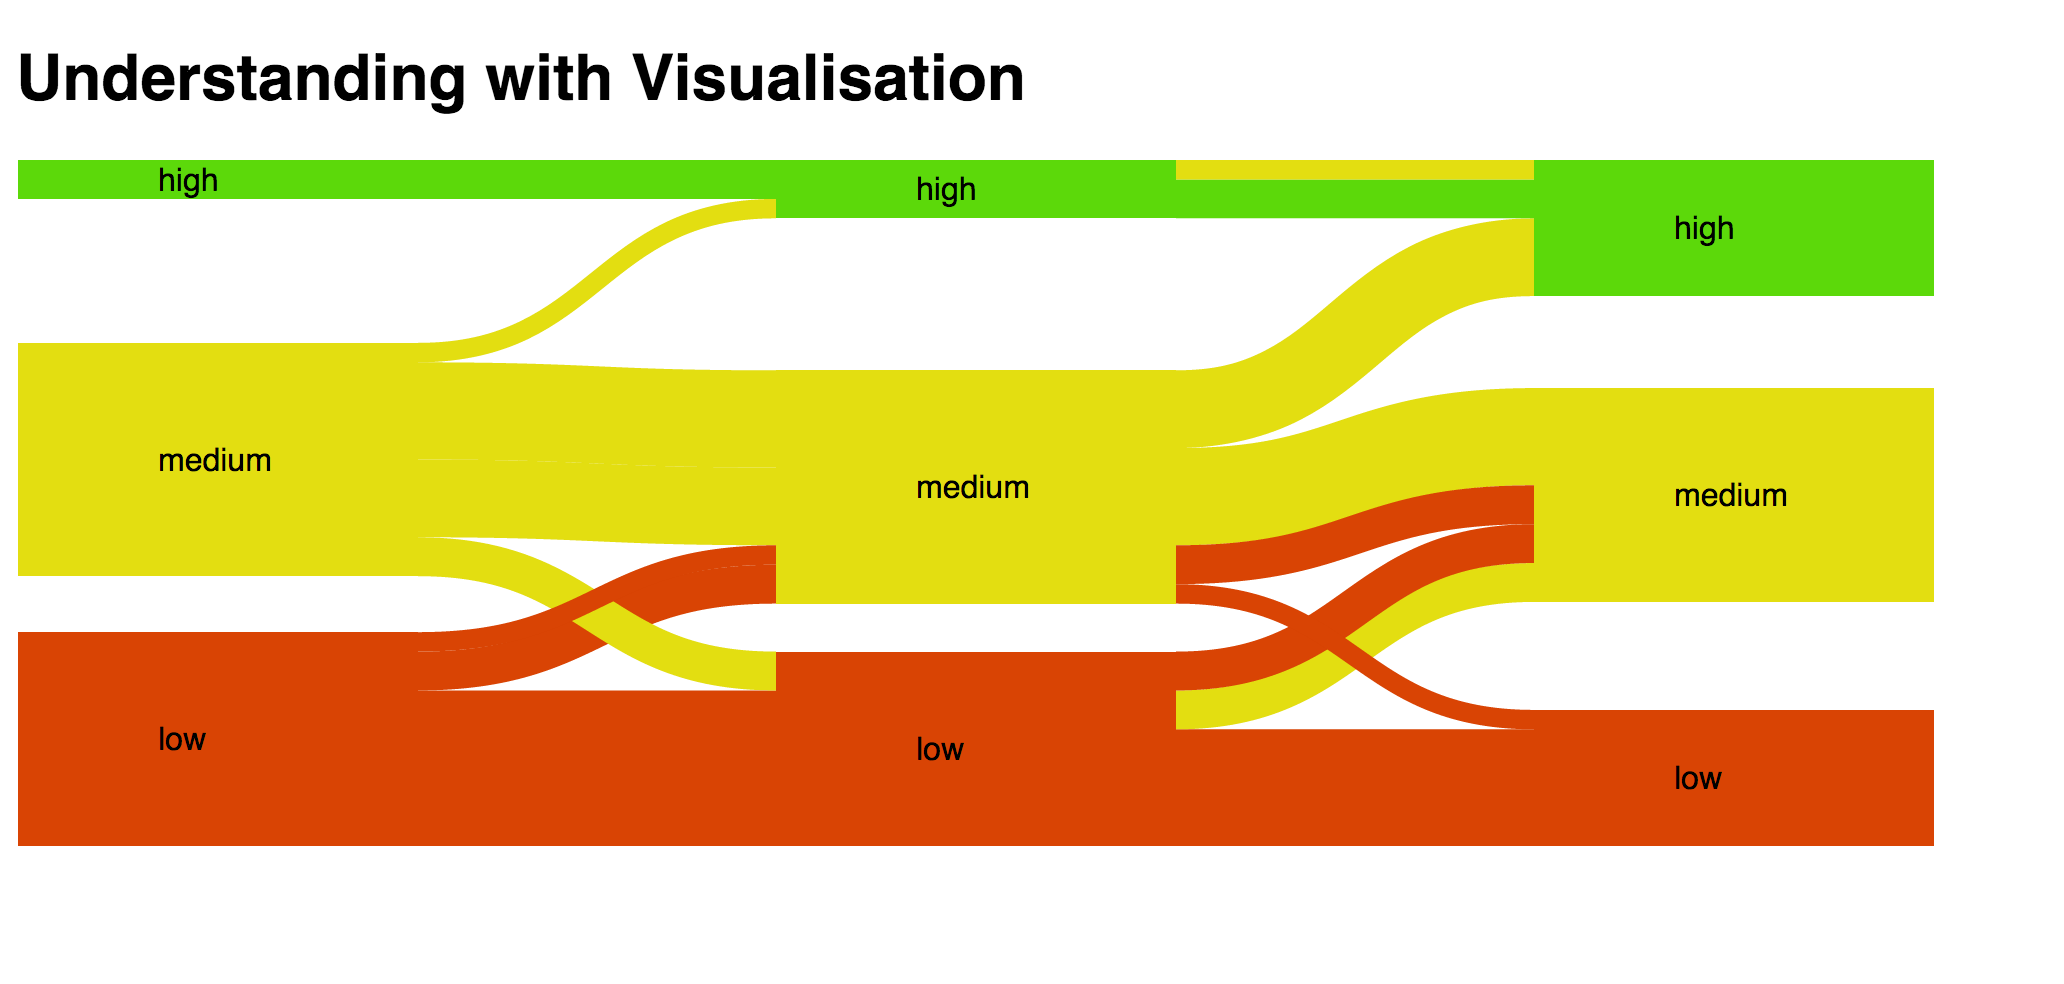
\includegraphics[width=\columnwidth]{../study-3/results/understanding-with-visualisation-study-3}
  \caption{Audience reported understanding during the beginning, middle and end of the performance with visualisations.}
  \label{fig:visualisations-understanding}
\end{figure}

\clearpage}

\section{Discussion}




\subsection{Validity}

A number of factors were identified that could influence the validity of the user study results.

Due to a technical oversight during the first performance, the visualisation underlay was difficult to distinguish. 
% This was this was intentionally left the same for the second performance group.

A large proportion of the audience stated that they had coding experience. An audience experienced in coding may be less interested in viewing visualisations and have a preference for viewing code directly.

\subsection{Limitations}

-this set of visualisations again suffered from being obscured by the code displayed on the screen, however, compared to the second study the visualisations were logically placed in relation to the source code... from top to bottom, in function order.


\section{Summary}










